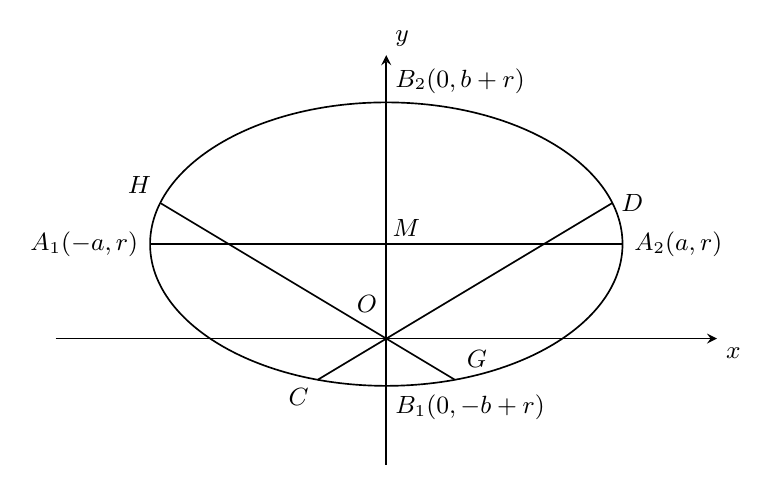
\begin{tikzpicture}[scale=1,line width=.6pt]
\tikzset{lbl/.style={font=\small,inner sep=1pt}}
% axes
\draw[->,>=stealth] (-4.2,0)--(4.2,0) node[lbl,below right=2pt] {$x$};
\draw[->,>=stealth] (0,-1.6)--(0,3.6) node[lbl,above right=2pt] {$y$};
% ellipse center M(0,1.2), a=3, b=1.8 : x^2/9+(y-1.2)^2/3.24=1
\draw (0,1.2) ellipse (3 and 1.8);
% long axis A1A2 at y=1.2
\draw ( -3,1.2)--(3,1.2);
% lines through origin: C-D (positive slope), H-G (negative slope)
\coordinate (D) at (2.8708286934,1.7224972160);
\coordinate (C) at (-0.8708286934,-0.5224972160);
\draw (C)--(D);
\coordinate (H) at (-2.8708286934,1.7224972160);
\coordinate (G) at (0.8708286934,-0.5224972160);
\draw (H)--(G);
\node[lbl,left=3pt] at (-3,1.2) {$A_{1}(-a,r)$};
\node[lbl,right=3pt] at (3,1.2) {$A_{2}(a,r)$};
\node[lbl,above right=2pt] at (0,3.0) {$B_{2}(0,b+r)$};
\node[lbl,below right=2pt] at (0,-0.6) {$B_{1}(0,-b+r)$};
\node[lbl,right=3pt,xshift=-2pt,yshift=6pt] at (0,1.2) {$M$};
\node[lbl,above left=3pt,xshift=1pt,yshift=5pt] at (0,0) {$O$};
\node[lbl,below left=2pt] at (C) {$C$};
\node[lbl,right=2pt] at (D) {$D$};
\node[lbl,above left=2pt] at (H) {$H$};
\node[lbl,above right=3pt] at (G) {$G$};
\end{tikzpicture}